\documentclass[a4paper,12pt]{article}
\usepackage[a4paper,top=1.3cm,bottom=2cm,left=1.5cm,right=1.5cm,marginparwidth=0.75cm]{geometry}
\usepackage{cmap}
\usepackage{mathtext}
\usepackage[T2A]{fontenc}
\usepackage[utf8]{inputenc}
\usepackage[english,russian]{babel}
\usepackage{siunitx}
\usepackage{enumitem}
\usepackage{placeins}

\usepackage{graphicx}

\usepackage{wrapfig}
\usepackage{tabularx}
\usepackage{multirow}

\usepackage{amsmath,amsfonts,amssymb,amsthm,mathtools} 
\usepackage{float} 
\usepackage{wasysym}
\usepackage{fourier} 
\usepackage{array}


\usepackage{physics}
\usepackage{caption}
\usepackage{subcaption}


\usepackage[rgb]{xcolor}
\usepackage{icomma} 
\usepackage{euscript}
\usepackage{mathrsfs}
\usepackage{enumerate}
\usepackage{graphicx}
\usepackage{cmap}									
\usepackage{tabularx}

\usepackage{alltt}
\usepackage{psvectorian}
\usepackage{listings}

\usepackage{hyperref}
\usepackage[rgb]{xcolor}
\hypersetup{
colorlinks=true,urlcolor=blue
}
\usepackage{amsmath,amsfonts,amssymb,amsthm,mathtools}
\usepackage{icomma}
\mathtoolsset{showonlyrefs=false}
\usepackage{euscript}
\usepackage{mathrsfs}
\DeclareMathOperator{\sgn}{\mathop{sgn}}
\newcommand*{\hm}[1]{#1\nobreak\discretionary{}
{\hbox{$\mathsurround=0pt #1$}}{}}

%%% Заголовок
\author{Макаров Лев Евгеньевич}
\title{Лабораторная работа №3.7.1

Скин-эффект
}
\date{\today}

\begin{document}

\begin{titlepage}
	\begin{center}
		{\large МОСКОВСКИЙ ФИЗИКО-ТЕХНИЧЕСКИЙ ИНСТИТУТ (НАЦИОНАЛЬНЫЙ ИССЛЕДОВАТЕЛЬСКИЙ УНИВЕРСИТЕТ)}
	\end{center}
	\begin{center}
		{\large Физтех-школа фотоники, электроники и молекулярной физики}
	\end{center}
	
	
	\vspace{4.5cm}
	{\huge
		\begin{center}
			{\bf Отчёт о выполнении лабораторной работы 3.7.1}\\
			Скин-эффект
		\end{center}
	}
	\vspace{2cm}
	\begin{flushright}
		{\LARGE Автор:\\ Макаров Лев Евгеньевич \\
			\vspace{0.2cm}
			Б04-306}
	\end{flushright}
	\vspace{8cm}
	\begin{center}
		Долгопрудный 2024
	\end{center}
\end{titlepage}

\textbf{Цель работы:} 
\begin{enumerate}
	\item исследовать явление проникновение переменного магнитного поля в медный полый цилиндр
\end{enumerate}

\textbf{В работе используются:} 
\begin{itemize}
    \item генератор сигналов АКИП–3420
    \item соленоид
    \item намотанный на полый цилиндрический каркас
    \item медный экран в виде полого цилиндра
    \item измерительная катушка
    \item амперметр
    \item вольтметр
    \item двухканальный осциллограф GOS–620
    \item RLC-метр
\end{itemize}
\medskip

\section{Теоретические сведения}
\subsection{Скин-эффект для полупространства}

\begin{wrapfigure}{r}{0.3\textwidth}
    \begin{center}
        \includegraphics[width=0.2\textwidth]{poluprostranstvo.png}
    \end{center}
\end{wrapfigure}

Рассмотрим квазистационарное поле внутри проводящей среды в простейшем плоском случае.
Пусть вектор $\vb*{E}$ направлен всюду вдоль оси $y$ и зависит только от координаты $x$, т. е. ${E_x} = {E_z} \equiv 0$, $E_y=E_y(x,t)$.
В квазистационарном приближении 
\begin{equation}
    \grad \times \vb*{H} = \sigma \vb*{E}
\end{equation}

Преобразуя это уравнение, можно получить уравнение, схожее с уравнением диффузии:
\begin{equation}
    \grad^2\vb*{H}=\sigma\mu\mu_0 \frac{\partial \vb*{H}}{\partial t}\label{eq:laplacian_H}
\end{equation}
Точно такое же уравнение имеет место и для вектора $E:$
\begin{equation}
    \grad^2\vb*{E}=\sigma\mu\mu_0 \frac{\partial \vb*{E}}{\partial t}\label{eq:diffusion}
\end{equation}

Подставляем в (\ref{eq:diffusion}) наше электрическое поле $E_y=E_y(x,t)$
\begin{equation}
    \frac{\partial^2 E_y}{\partial x^2} = \sigma\mu\mu_0\frac{\partial E_y}{\partial t}
    \label{eq:diffusion_chastni}
\end{equation}
Если $E_y(0,t)=E_0 e^{i\omega t}$ то решением (\ref{eq:diffusion_chastni}) будет функция вида
\begin{equation}
    E_y(x,t)=E_0 e^{-x/\delta} e^{i(\omega t - x/\delta)}
    \label{eq:skin_effect_poluprostranstvo}
\end{equation}
где
\begin{equation}
    \delta = \sqrt{\frac{2}{\omega\sigma\mu\mu_0}}
    \label{eq:delta}
\end{equation}
\subsection{Скин-эффект в тонком полом цилиндре}
\vspace{1cm}
\begin{wrapfigure}[36]{r}{0.3\textwidth}
    \begin{center}
        \includegraphics[width=0.28\textwidth]{cilindr}
    \end{center}
    \caption{Эл-магнитные поля в цилиндре}\label{fig:cilindr}
    
    \begin{center}
        \includegraphics[width=0.28\textwidth]{stenka}
    \end{center}
    \caption{Стенка цилиндра}\label{fig:stenka}
\end{wrapfigure}

Перейдем теперь к описанию теории в нашей работе. Из соображении симметрии и 
непрерывности соответствующих компонент векторов $\vb*{E}$ и $\vb*{H}$ можем сказать что
\begin{equation}
    H_z = H(r)e^{i\omega t} \text{, } E_\varphi = E(r)e^{i\omega t}
\end{equation}
и при этом функции $H(r)$ и $E(r)$ непрерывны.

Внутри цилиндра токов нет, следовательно $H(r)=H_1=\text{const}$ внутри цилиндра.
По теореме об электромагнитной индукции
\begin{equation}
    E(r) = -\frac{1}{2}\mu_0 r \cdot i \omega H_1
\end{equation}
откуда мы получаем граничное условие
\begin{equation}
    E_1=E(a)= -\frac{1}{2}\mu_0 a \cdot i \omega H_1
    \label{eq:granichnoe_uslovie_E}
\end{equation}

В приближении $h \ll a$ можем пренебречь кривизной стенки и смоделировать 
его бесконечной полосой. Тогда, надо решить уравнение (\ref{eq:laplacian_H})
с граничными условиями. Решая уравнение получим связь полей $H_1$ 
(поле внутри цилиндра которое мы будем измерять) и $H_0$, которое колеблется с частотой
$\omega$

\begin{equation}
    H_1 = \frac{H_0}{\ch(\alpha h) + \frac{1}{2} \alpha a \sh(\alpha h)} 
    \text{\ \ \ }
    \alpha = \sqrt{i\omega \sigma \mu_0} = \frac{\sqrt{2}}{\delta}e^{i\pi/4}
    \label{eq:svyaz_poley}
\end{equation}

из этой формулы получим сколько по фазе отстает поле $H_1$ от $H_0$.\\
При $\delta \gg h$ (низкочастотная область)
\begin{equation}
    \dfrac{|H_1|}{|H_0|} = \dfrac{1}{\sqrt{1+ \frac{1}{4} (a h \sigma \mu_0 \omega )^2 }}
    \label{eq:H_low_freq}
\end{equation}
\begin{equation}
    \tg \psi \approx \frac{ah}{\delta^2} = \pi a h \sigma \mu \mu_0 \nu
    \label{eq:faza_low_freq}
\end{equation}

При $\delta \ll h$
(высокочастотная область)
\begin{equation}
    \dfrac{H_1}{H_0} = \dfrac{4}{2+\alpha a}e^{-\alpha h} \approx \dfrac{2 \sqrt{2} \delta}{a} e^{\frac{h}{\delta}}e^{-i \left( \frac{\pi}{4} + \frac{h}{\delta}\right)}
\end{equation}
\begin{equation}
    \psi \approx \frac{\pi}{4} + \frac{h}{\delta} = 
    \frac{\pi}{4} + h \sqrt{\frac{\omega \sigma \mu_0}{2}}
    \label{eq:faza_high_freq}
\end{equation}

\newpage 	
\subsection{Установка и процесс измерения}
\begin{wrapfigure}{l}{0.5\textwidth}
    \begin{center}
        \includegraphics[width=0.45\textwidth]{ustanovka}
    \end{center}
    \caption{Установка}\label{fig:ustanovka}
\end{wrapfigure}

Переменное магнитное поле создается соленоидом 1, на который подается переменный ток со звукового генератора ЗГ. Внутри соленоида расположен медный экран 2. Магнитное поле внутри цилиндра измеряется катушкой 3. Напряжение на катушке пропорциональна производной $\dot{B_1}(t)$
\begin{equation*}
    U(t) \propto \dot{B_1}(t) = -i\omega H_1 e^{i\omega t}
\end{equation*}
Поле внутри цилиндра пропорциональна току через соленоид
\begin{equation*}
    H_0(t) \propto I(t)
\end{equation*}
Отсюда несложно увидеть, что
\begin{equation}
    \frac{\abs{H_1}}{\abs{H_0}} = c \cdot \frac{U}{\nu I} = \xi_0 \xi
    \label{eq:otnoshenie_amplitud}
\end{equation}
где константу  $\xi_0$ можно определить из условия $\abs{H_1}/\abs{H_0} \rightarrow 1$ при
$\nu \rightarrow 0$.\\

При измерениях разности фаз нужно учесть, что первый сигнал на осциллографе
пропорционален магнитному полю снаружи, а второй пропорционален производному
поля внутри цилиндра по времени, поэтому измеренная на осциллографе разность фаз $\varphi$ будет на $\frac{\pi}{2}$ больше реальной $\psi$:
\[\varphi = \psi + \frac{\pi}{2}\]
\subsection{Влияние скин-эффекта на индуктивность катушки}
Рассмотрим магнитный поток через катушку как сумму двух магнитных потоков: 1)пронизывающий область между катушкой и цилиндрическим экраном $\Phi_{out}$; 2) пронизывающий область за экраном $\Phi_{in}$:
\begin{equation}
    \Phi = \Phi_{out} + \Phi_{in} = H_0 S_0 + H_1 S_1 = L I
\end{equation}
Очевидно, что минимальная индуктивность будет в случае, когда $\Phi_{in} = 0$ (поле есть только во внешней области). При этом $L_{min}$ не зависит от частоты:
\begin{equation}
    L_{min}  = \dfrac{\Phi_{out}}{I} \quad \Phi_{in} = H_1 S_1 = \dfrac{H_1 S_1}{H_0 S_0} \Phi_{out} = \dfrac{\Phi_{out}}{n} \dfrac{S_1}{S_0}
\end{equation}
\begin{equation}
    n = \dfrac{H_0}{H_1} = \dfrac{|H_0|}{|H_1|} \dfrac{1}{\cos (\psi)}
\end{equation}
\begin{equation}
    \Phi_{max} = \Phi_{out} + \Phi_{in_{max}} = H_0(S_0 + S_1 ) = L_{max} I_m
\end{equation}
\begin{equation}
    L = L_{min} + \dfrac{L_{max} - L_{min} }{n}
\end{equation}
\begin{equation}
    \dfrac{L_{max} - L_{min}}{L - L_{min}} = (\pi a h \mu_0 \sigma \nu)^2
\end{equation}

\section{Результаты измерений и обработка данных}


\section{Ход работы}

Параметры медного цилиндра:\\
$D = 45$ мм -- наружный диаметр\\
$h = 1.5$ мм -- толщина стенки.\\
Использовав табличные значения рассчитаем критическую частоту при которой $ h = \delta$
$$
\nu_h = \dfrac{1}{\pi \mu_0 \sigma h^2} \approx 2252 \text{ Гц}
$$

\subsection{Измерения амплитуд в области низких частот}


Воспользуемся формулой \eqref{eq:H_low_freq} для скин-слоя при низких частотах
\begin{equation}
    \left(\dfrac{|H_1|}{|H_0|}\right)^2 = \dfrac{1}{1+ \frac{1}{4} (a h \sigma \mu_0 \omega )^2 } = \xi^2 \xi_0^2
\end{equation}
Где $\xi = \dfrac{U}{I\nu}$
\begin{equation}
    \dfrac{1}{\xi^2} = (\xi_0\nu\pi a h \sigma \mu_0)^2 + \xi_0^2
\end{equation}
Построим график $\frac{1}{\xi^2} = f(\nu^2)$, по МНК найдём коэффициенте $\xi_0$ и $\sigma$.


$$
\dfrac{1}{\xi^2} = k\nu^2 + \xi_0^2
$$

$$
k = \frac{\langle Y X\rangle - \langle Y \rangle \langle X \rangle}{\langle X^2 \rangle - \langle X \rangle^2}
$$

$$
\xi_0^2 = \langle Y \rangle - k \langle X \rangle
$$ 

Найдём случайную погрешность $\sigma_{k}$:\\
Погрешность коэффициента можно вычислить по формуле:
$$
\sigma_{k} = \frac{1}{\sqrt{N-2}}\sqrt{\frac{\langle (Y)^2 \rangle - \langle Y \rangle ^2}{\langle X^2 \rangle - \langle X \rangle ^2} - k^2}
$$
$$
\sigma_{\xi_0^2} = \sigma_k \sqrt{\langle X^2 \rangle}
$$

$$
    \xi_0 =  (71 \pm 6) \dfrac{\text{Гц}}{\text{Ом}} 
    \qquad \sigma = (4.36 \pm 0.22) \cdot 10^7 \dfrac{\text{См}}{\text{м}}
$$


\begin{figure}[H]
    \centering
    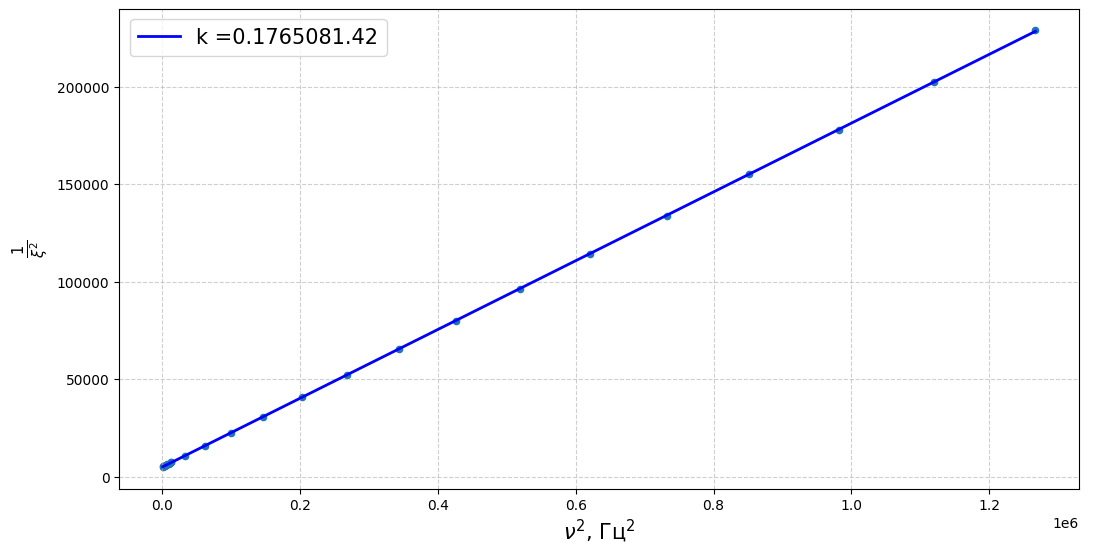
\includegraphics[width=1\textwidth]{1_grf}
    \caption{График зависимости $\dfrac{1}{\xi^2}(\nu^2)$}
    \label{1.1}
\end{figure}

\subsection{Измерение проводимости через разности фаз при низких частотах}
Построим график зависимости $\tg(\psi) = f(\nu)$\\ 
По МНК определим коэффициент проводимости меди
\begin{figure}[H]
    \centering
    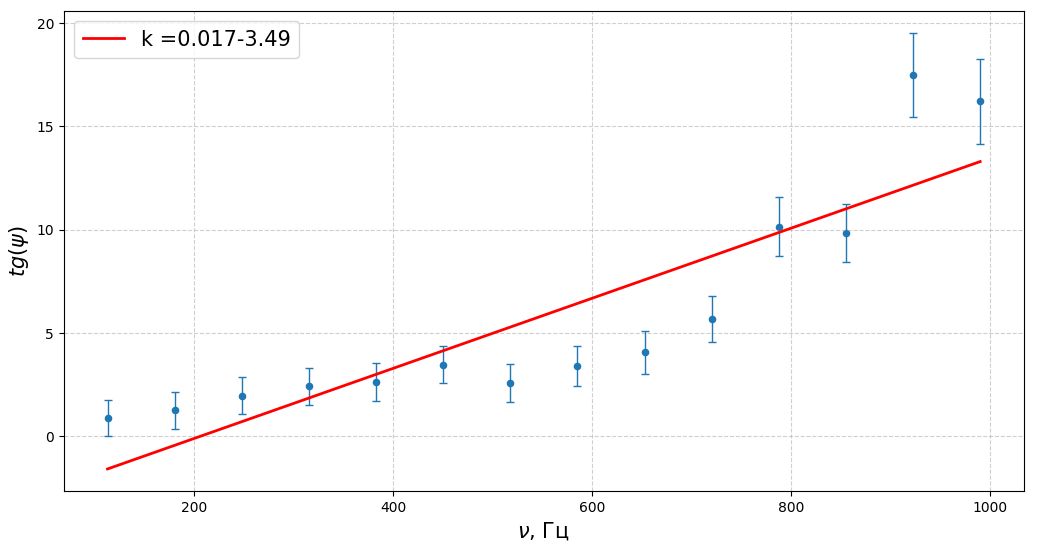
\includegraphics[width=1\textwidth]{2_grf}
    \caption{График зависимости $\tg (\psi) = f(\nu)$}
    \label{1.2}
\end{figure}
$$
k = \pi a h \mu_0 \sigma = 0.017 \text{, c} \qquad \sigma = \dfrac{k}{\pi a h \mu_0} = 7.61 \pm 0.54 \cdot 10^7 \dfrac{\text{См}}{\text{м}}
$$

\subsection{Измерение проводимости через разность фаз в высокочастотном диапазоне}
По формуле (14), при $\delta \ll h$
$$
\psi - \dfrac{\pi}{4} = k \cdot \sqrt{\nu} \quad k = h \sqrt{\pi \mu_0 \sigma} = 0.023 \pm 0.001 
$$

\begin{figure}[H]
    \centering
    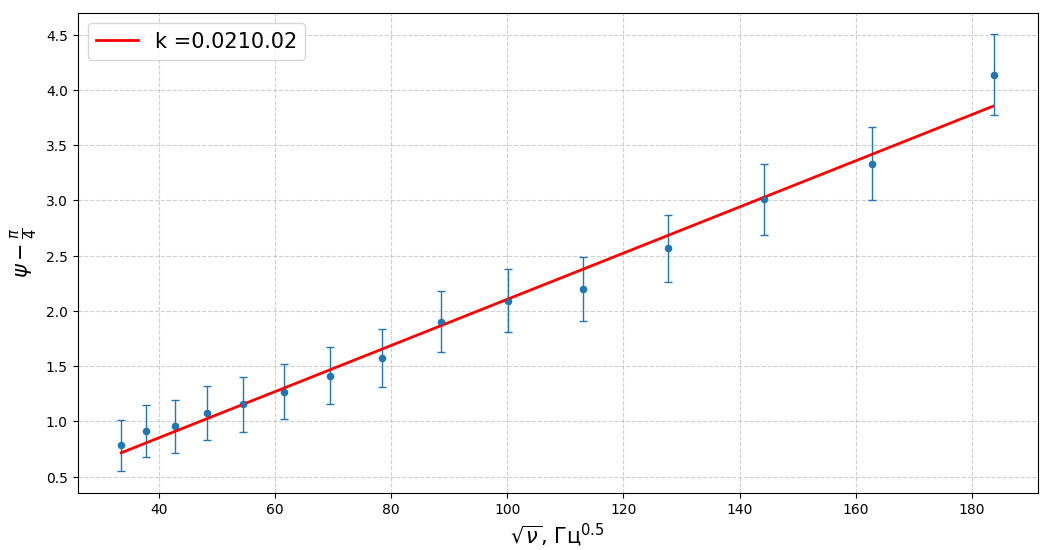
\includegraphics[width=1\textwidth]{3_grf}
    \caption{График зависимости $\tg (\psi) = f(\nu)$}
    \label{1.3}
\end{figure}
$$
\sigma = 6.09 \pm 0.31 \cdot 10^{7} \dfrac{\text{См}}{\text{м}}
$$

\subsection{Измерение проводимости через изменение индуктивности}
 Измерить проводимость можно также через изменение индуктивности катушки внутри цилиндра. Данные, измеренные с помощью RCL-метра:
 \begin{table}[!ht]
    \centering
    \begin{tabular}{|l|l|l|l|l|l|l|l|l|l|l|}
        \hline
        L, мГн & 19 & 13.2 & 9 & 7.82 & 7.12 & 6.6 & 5.61 & 5.67 & 5.68 & 5.46 \\ \hline
        $\nu$ & 40 & 150 & 300 & 400 & 500 & 600 & 800 & 1500 & 2000 & 6000 \\ \hline
        L, мГн & 5.63 & 6.02 & 6.77 & 8.74 & ~ & ~ & ~ & ~ & ~ & ~ \\ \hline
        $\nu$ & 12000 & 16200 & 20000 & 25000 & ~ & ~ & ~ & ~ & ~ & ~ \\ \hline
    \end{tabular}
 \end{table}
 Построим график $L(\nu)$
    \begin{figure}[H]
    \centering
    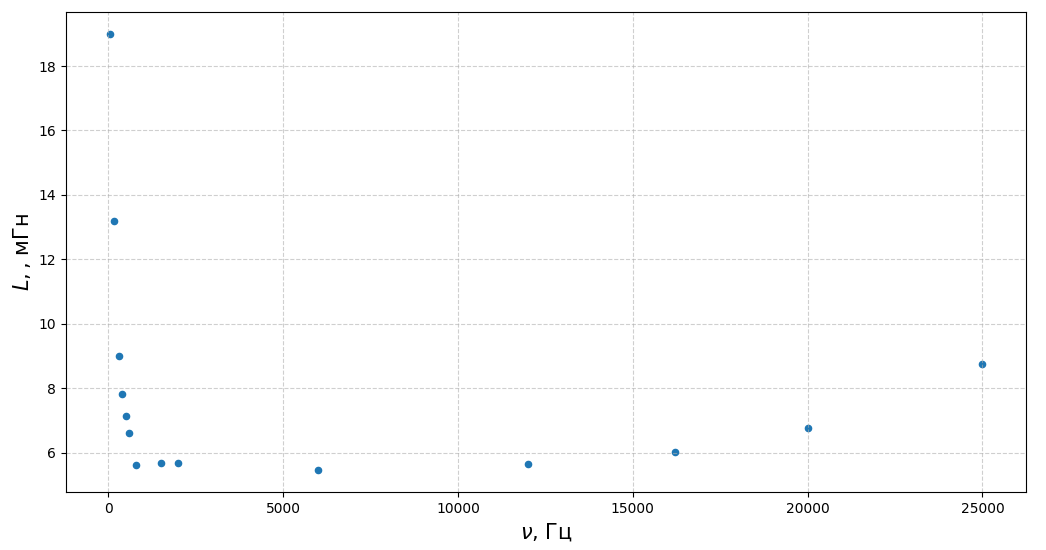
\includegraphics[width=1\textwidth]{4_grf}
    \caption{График зависимости $L(\nu)$}
    \label{1.4}
 \end{figure}
 Полученные максимальные и минимальные значения индуктивности $L_{min} = 5.46$ мГн, $L_{max} = 19$ мГн\\
 по формуле (21)
 $$
    \dfrac{L_{max} - L_{min}}{L - L_{min}} = (\pi a h \mu_0 \sigma \nu)^2
 $$
 получается коэффициент наклона графика
 $$
    k = (\pi a h \mu_0 \sigma )^2 \qquad \sigma = \dfrac{\sqrt{k}}{\pi a h \mu_0}
 $$
\begin{figure}[H]
    \centering
    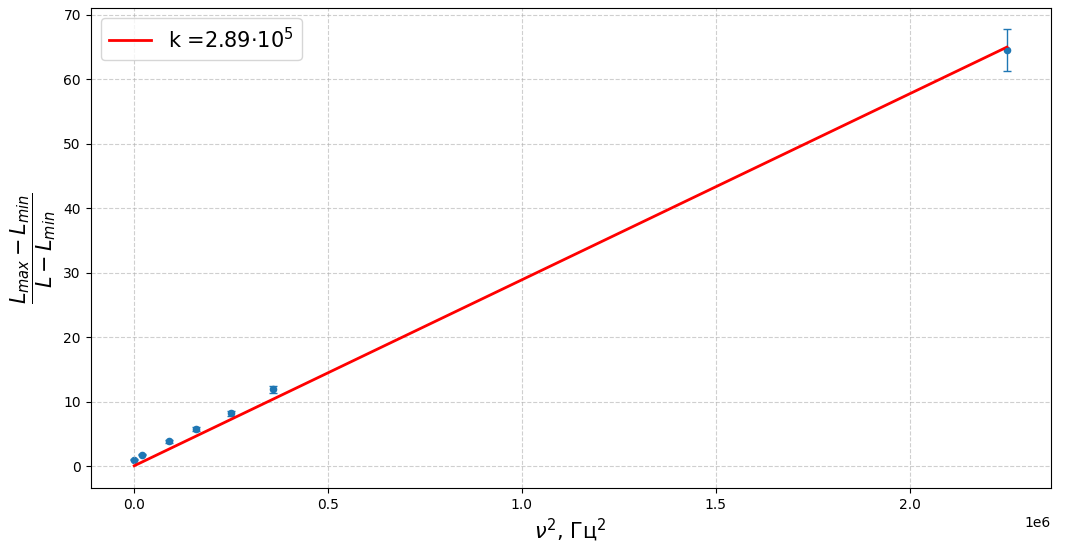
\includegraphics[width=1\textwidth]{5_grf}
    \caption{График зависимости $\dfrac{L_{max} - L_{min}}{L - L_{min}} = f(\nu^2)$}
    \label{1.5}
 \end{figure}
 $$
 \sigma = 4.6 \pm 0.1 \cdot 10^7 \dfrac{\text{См}}{\text{м}}
 $$
 Построим график для $\frac{|H_1|}{|H_0|}$, для теоретических значений и полученный приблежений при низких частотах и высоких частотах\\
 
 Формула для теоретических значений, где $x = \dfrac{h}{\delta}$
 \begin{equation}
    \frac{|H_1|}{|H_0|} = \dfrac{1}{\sqrt{ \left( \ch(x) \cos(x) + \frac{1}{2\delta} a \sh(x) \cos(x) \right)^2 + \left( \sh(x) \sin(x) + \frac{1}{2\sigma} a \ch(x) \sin(x) \right)^2  }}
 \end{equation}

 \begin{figure}[H]
    \centering
    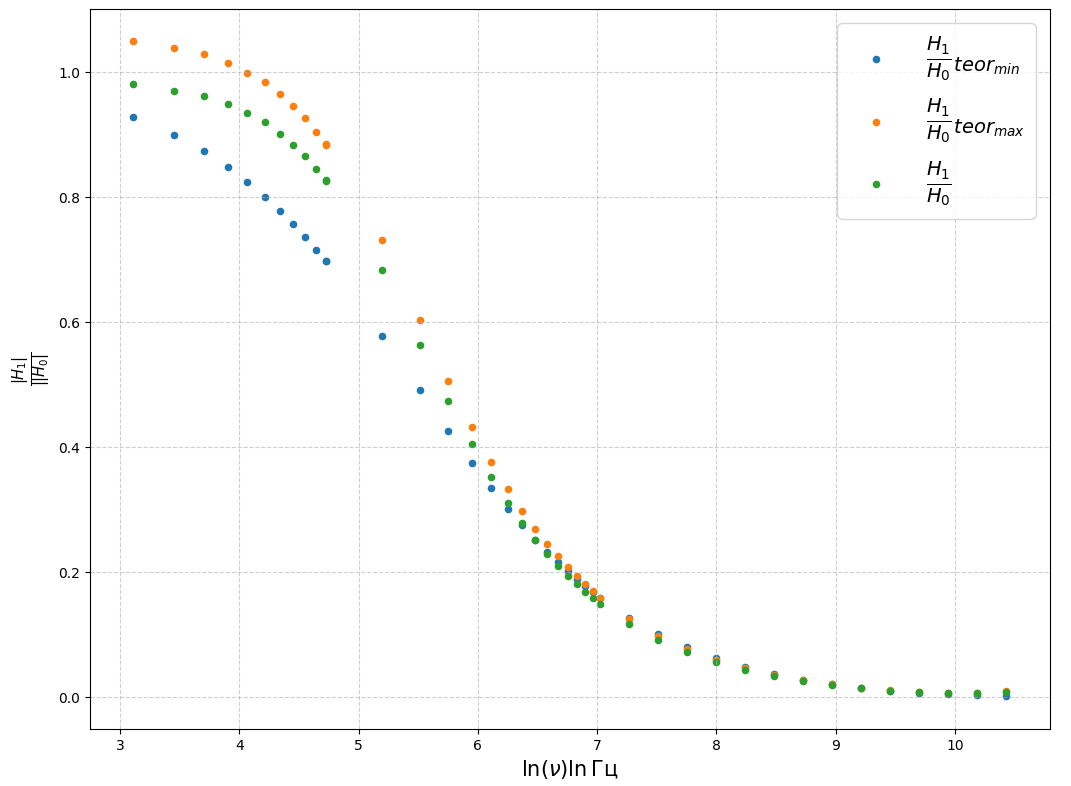
\includegraphics[width=1\textwidth]{7_grf}
    \caption{График зависимости  $\frac{|H_1|}{|H_0|}(\nu)$}
    \label{1.7}
 \end{figure}
 
 \section{Вывод}
 \begin{table}[!ht]
    \centering
    \begin{tabular}{|l|l|l|l|}
        \hline
        N & 1 & 2 & 3 \\ \hline
        $\sigma $ & 4.36$\pm$0.22 & 7.61$\pm$0.54 & 4.6$\pm$0.1 \\ \hline
    \end{tabular}
 \end{table}





\end{document}
